\begin{exercise}\label{ex:1chap1}
Let $P=[p:q:r] $ be an interior point of an equilateral triangle $T=ABC$.

\noindent i) Show that the distances of $P$ to the sidelines of the triangle $T$ are given by
\[ [pk,qk,rk], \;\;\;k=\frac{2\Delta}{pa+qb+rc}\]
where $\Delta$ is the area of the triangle.

 \noindent ii)
 Show that  $k(p+q+r)$ is equal to the length of the triangle's altitude, i.e., the sum is independent of the position of the point.
 
 \noindent iii) Show that the same result is true when $P$ is an exterior point, but here we need to consider distances with signal, according to the position of $P$. See \cref{fig:trilinear_signal}.
 
 \noindent iv) Show that the reciprocal is true, i.e., if the sum of distances is independent of the point, then the triangle is equilateral.
 
 \noindent iv) Generalize items ii), iii) and iv)  for regular polygons.
 \end{exercise}
 
 \begin{exercise}\label{ex:2chap1} Show that $X_i$??  of the reference triangle    is the symmedian point of its excentral triangle.
 
  \end{exercise}
 
  \begin{exercise}\label{ex:3appA}
 Let $ABC$ be a  triangle and    $P$ and $Q$ be isogonal conjugates.  Then the circumcenters of the triangles $BPC$ and $BQC$ are inverses with respect to the circumcircle of the triangle $ABC$.
   \end{exercise}
  
   \begin{exercise}\label{ex:4appA}
   Let $P$ and $Q$ be isogonal conjugates in the interior of
the triangle $ABC$. Then the   pedal  triangles of $P$ and $Q$
 share a circumcircle. Moreover, the center of this circle is the midpoint
of $PQ$.
    \end{exercise}
   
      \begin{exercise}\label{ex:5app}
  Let $P $ and $Q$ isogonal conjugates.  If the point
is reflected about the sides
$AB$, $BC$ and $AC$.
  Then the resulting triangle has circumcenter the point $P$.
 
    \end{exercise}  \begin{exercise}\label{ex:6app}
  Let $\mathcal{E}$ be an ellipse inscribed in a triangle $ABC$. Then foci $F_1$ and $F_2$ of $\mathcal{E}$ are isogonal conjugates. 
 
    \end{exercise}
    
     \begin{exercise}\label{ex:7app}
 Consider two lines $x$ and $y$ passing through $P_0$.
 Let $ u$ and $v$ conjugate lines with respect to $x$ and $y$. Let $P\in u$ and $P_x\in x$ and $P_y\in y$ the pedal points of $P$. 
 
 \noindent i) Show that the points $\{P_0,P,P_x,P_y\} $
 are con-cyclic.
 
 \noindent ii) Show that the line $h=P_xP_y$ is orthogonal to the line $v$. See \cref{fig:isogonal_orthogonal}. 
 
 \begin{figure}[H]
    \centering
   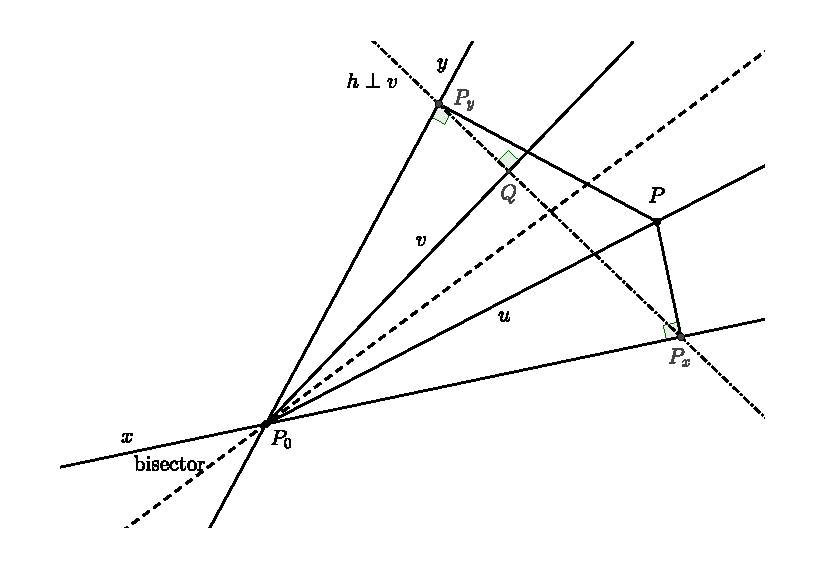
\includegraphics[scale=0.7]{pics_appA_0910_isogonal_ortogonal_conjugateline.pdf}
    \caption{ Isogonal line $v$ is orthogonal to  $h=P_xP_y$.
    \label{fig:isogonal_orthogonal}
    }
\end{figure}
 
    \end{exercise}
    
         \begin{exercise}\label{ex:8app}
         Show that the Brocard points can be  constructed as shown in \cref{fig:brocard_construction}.
         
         Consider a triangle $ABC$ and draw a line passing through $A$ and parallel to $BC$. Consider also a circle passing through $C$ and tangent to the line $AB$ at the vertex $A$. The point $D$ is the intersection of the line and circle constructed above.  The line $BD$ intersect the circle at the Brocard point $\Omega_1$ of $ABC$. Repeat this construction for the other vertices and obtain $\Omega_2.$
     
 \begin{figure}[H]
    \centering
   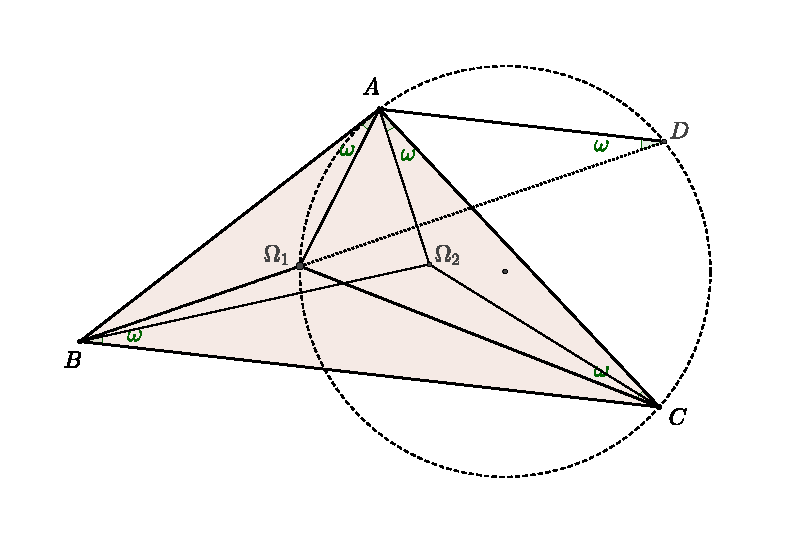
\includegraphics[scale=0.7]{zappA/pics/pics_appA_0930_brocard_points_construcao.pdf}
    \caption{ Geometric construction of Brocard points
    \label{fig:brocard_construction}
    }
\end{figure}
 
    \end{exercise}